\chapter{Helicity Corelated Pedestal Analysis}
%\chapter{HELICITY CORRELATED PEDESTAL ANALYSIS}
\label{Helicity Corelated Pedestal Analysis 2}


%%%%%%%%%%%%%%%%%%%%%%%%%%%%%%%%%%%%%%%%%%%%%%%%%%%%%%%%%%%%%%
\section{Helicity Corelated Pedestal Analysis\index{Helicity!Helicity Corelated Pedestal Analysis}}

Helicity is the projection of the spin $\vec{S}$ onto the direction of momentum\index{Helicity!Helicity}.

\begin{equation} \label{equ:helicity1}
\vec{h} = \vec{J} \cdot \hat{p} = \vec{L} \cdot \hat{p} + \vec{S} \cdot \hat{p} = \vec{S} \cdot \hat{p} 
\end{equation}



\subsection{Condition of Experimental Data Taking}
\label{Condition of Experimental Data Taking}

\begin{itemize}
\item Dedicated pedestal runs: Typically 5~minutes dedicated beam off pedestal run were taken with production running once a day during Run 1 and once a shift during Run 2. There were also $\sim$1~hour long beam off pedestal runs taken throughout, whenever there was an opportunity.
\item Target - LH2 , Al, No target: Most of the pedestal runs are with LH2 target, but there were significant number of Al pedestal runs. There were few runs without target and while the target was moving.
\item Beam OFF: Only beam off pedestal runs were included in this analysis. There were several runs marked as pedestal in the HCLOG that didn't pass the standard beam current cuts (details in~\ref{Condition of This Analysis}), meaning they had some beam and hence were excluded from this analysis. More details has been presented in~\cite{presentation:nur_hel_cor_ped_talk1, presentation:nur_hel_cor_ped_talk2}.
\end{itemize}



%-------------------------------------------%
\subsection{Condition of This Analysis}
\label{Condition of This Analysis}

\begin{itemize}
\item Analyzer version: 4024 (12th February 2012 14:06:42).
\item Beam current cut (global): -10 to 1 $\mu$A.
\item Effective charge cut (global) on BPM 3h09 and 3c12: -100000 to 25000.
\item Turned OFF normalization: The main detectors and luminosity monitors are normalized to the charge monitors for nominal parity analysis so it is important that neither have any evidence of helicity correlated pedestal differences. Hence, MD and Lumi normalization were turned off during pedestal analysis.
\item Hel\_Tree and Mps\_Tree: Helicity correlated differences were taken from Hel\_Tree and raw pedestal signal from Mps\_Tree.
\item Turned OFF Data Base update.
\item Turned OFF blinding factor for this analysis keeping the integrity of the experiment.~\cite{pking}
\end{itemize}

%-------------------------------------------%
\subsection{Configuration}
\label{Configuration}

The following command has been used for this analysis using standard Q-weak analyzer.
\begin{equation} \label{equ:eqAnalysis1}
\texttt{qwparity -r 18974  -c pedestal\_ifarm.conf}\\
\end{equation}

%\noindent
Here, 18974 is the run number and pedestal\_ifarm.conf is the configuration file and has following configurations:

\noindent
\texttt{chainfiles = yes\\
single-output-file = yes\\
detectors = detectors$\_$pedestal.map\\
codafile-stem = QwRun$\_$\\
codafile-ext = log\\
QwMainCerenkovDetector.normalize = no\\
QwLumi.normalize = no\\
rootfile-stem = Qweak$\_$Hel$\_$Ped$\_$Ana$\_$\\
enable-differences = yes\\
disable-histos = yes\\
blinder.force-target-out = yes\\
disable-slow-tree = yes\\
disable-burst-tree = yes\\
disable-by-type = QwScanner\\
disable-by-type = QwBeamMod\\
enable-tree-trim = yes\\
%tree-trim-file = pedestal_tree_trim.in\\
QwDatabase.accesslevel = OFF\\}

\subsection{List of Variables}
\label{List of Variables}
The list of variables included in this analysis are shown below. The variables are from the Hel\_Tree of the standard analyzed rootfiles, and has the following nomenclature ``diff\_qwk\_VARIABLE\_NAME".

\subsubsection{Main Cerenkov Detector(17)}
\label{Main Cerenkov Detector}
mdallbars, md1pos, md2pos, md3pos, md4pos, md5pos, md6pos, md7pos, md8pos, md1neg, md2neg, md3neg, md4neg, md5neg, md6neg, md7neg, md8neg.

\subsubsection{Downstream Luminosity Detector(9)}
\label{Downstream Luminosity Detector}
dslumi$\_$sum, dslumi1, dslumi2, dslumi3, dslumi4, dslumi5, dslumi6, dslumi7, dslumi8.

\subsubsection{Uptream Luminosity Detector(9)}
\label{Upstream Luminosity Detector}
uslumi$\_$sum, uslumi1pos, uslumi3pos, uslumi5pos, uslumi7pos, uslumi1neg, uslumi3neg, uslumi5neg, uslumi7neg.

\subsubsection{Beam Current Monitor(9)}
\label{Beam Current Monitor}
charge\footnote{charge = bcm1+bcm2 for Run-I and = bcm8 for most of Run-II.}, bcm1, bcm2, bcm5, bcm6, bcm7, bcm8, bcmgl1, bcmgl2.\\

\subsection{List of Runs}
\label{List of Runs}
The list of dedicated pedestal runs included in this analysis are shown in following subsections. The data taken during 31 January 2011 - 17 May 2012.

\subsubsection{Wien 0}
\label{Wien 0}
9593
9546
9539
9510
9483
9469
9456
9436
9407
9394
9354
9353
9352
9314
9303
9288
9205
9131
9129
9098
9095
9067
9028
9027
9026

\subsubsection{Wien 1}
\label{Wien 1}
10182
10168
10150
10133
10105
10092
10087
10083
10082
10077
10066
10060
10026
9979
9972
9970

\subsubsection{Wien 2}
\label{Wien 2}
11123
11106
11089
11067
11066
11053
11050
11049
11032
10997
10974
10969
10954
10953
10945
10920
10916
10902
10892
10891
10890
10889
10887
10886
10822
10805
10802
10799
10797
10782
10781
10743
10730
10720
10716
10711
10708
10705
10702
10699
10288
10287
10252
10239
10229
10201

\subsubsection{Wien 3}
\label{Wien 3}
11380
11343
11304
11289
11285
11274
11264
11255
11246
11238
11229
11215
11211
11206
11189
11177
11166
11164
11160
11146
11131

\subsubsection{Wien 4}
\label{Wien 4}
11691
11690
11670
11668
11661
11648
11633
11608
11585
11574
11555
11529
11444
11422

\subsubsection{Wien 5}
\label{Wien 5}
11715
11712
11691
11690
11670
11668
11661
11648
11633
11608
11585
11574
11555
11529
11444
11422
11380
11343
11304
11289
11285
11274
11264
11255
11246
11238
11229
11215
11211
11206
11189
11177
11166
11164
11160
11146
11131
11130
11123

\subsubsection{Wien 6}
\label{Wien 6}
14209
14206
14205
14147
14125
14124
14120
14102
14091
14064
14063
14062
14061
14060
14059
14058
14057
14041
14040
14039
14038
14037
14036
14035
14034
14025
13987
13986
13971
13969
13968
13967
13966
13928
13927
13926
13925
13924
13914
13895
13888
13886
13859
13858

\subsubsection{Wien 7}
\label{Wien 7}
14683
14675
14674
14669
14631
14595
14568
14567
14564
14561
14552
14530
14529
14528
14527
14524
14466
14464
14452
14449
14440
14430
14384
14326
14325
14324
14322
14308

\subsubsection{Wien 8}
\label{Wien 8}
15980
15919
15913
15904
15888
15887
15877
15876
15817
15797
15766
15746
15708
15706
15699
15694
15676
15660
15659
15658
15657
15656
15645
15639
15638
15637
15624
15623
15618
15599
15591
15515
15514
15493
15488
15487
15420
15418
15417
15401
15400
15396
15395
15362
15359
15349
15338
15337
15321
15313
15311
15227
15247
15228
15214
15213
15176
15169

\subsubsection{Wien 9}
\label{Wien 9}
16207
16259
16329
16330
16368
16374
16387
16388
16391
16394
16395
16397
16398
16399
16400
16403
16404
16407
16420
16424
16425
16428
16446
16449
16454
16460
16465
16517
16518
16519
16520
16521
16522
16523
16581
16582
16583
16593
16595
16598
16606
16616
16619
16620
16626
16642
16643
16644
16719
16721
16736
16738
16739
16740
16742
16743
16764
16785
16797
16799
16810
16813
16814
16815
16816
16817
16818
16819
16830
16890
16907
16908
16909
16910
16911
16915
16921
16926
16934
16945
16950
16966
16967
16981
16988
16989
17000
17001
17002
17003
17004
17005
17006
17007
17018
17020
17021
17022
17023
17024
17028
17042
17043
17044
17045
17046
17047
17048
17049
17050
17051
17052
17093
17094
17095
17096
17097
17098
17099
17102
17103
17104
17105
17106
17107
17108
17109
17110
17144
17145
17146
17160
17165
17167
17173
17174
17190
17193
17194
17195
17200
17204
17222
17257
17284
17310
17332
17333
17346
17347
17348
17349
17350
17351
17352
17353
17354
17355
17356
17357
17358
17359
17360
17361
17362
17363
17364
17365
17366
17367
17368
17369
17374
17375
17399
17414
17460
17462
17464
17467
17469
17470
17631
17633
17634
17635
17636
17646
17650
17677
17682
17696
17708
17711
17715
17718
17723
17753
17801
17868
17869
17870
17890
17891
17957
17958
18001
18002
18003
18005
18028
18031
18043
18045
18069
18103
18115
18137
18150
18155
18160
18170
18179
18192
18206
18227
18230
18237
18259
18281
18288
18321
18327
18330
18373
18419
18422
18447
18448

\subsubsection{Wien 10}
\label{Wien 10}
18587
18588
18589
18590
18606
18611
18612
18644
18676
18677
18678
18679
18680
18681
18682
18683
18684
18685
18713
18719
18724
18727
18730
18733
18736
18739
18742
18743
18801
18815
18818
18831
18832
18847
18848
18851
18852
18855
18856
18863
18864
18865
18868
18869
18870
18871
18872
18874
18875
18876
18877
18878
18879
18880
18881
18885
18899
18900
18902
18909
18910
18928
18930
18935
18942
18944
18951
18952
18953
18972
18973
18974


%%%%%%%%%%%%%%%%%%%%%%%%%%%%%%%%%%%%%%%%%%%%%%%%%%%%%%%%%%%%%%
\section{Background Detectors}
\label{Background Detectors}

The helicity correlated differences from  Hel\_Tree and pedestal subtracted signals from Mps\_Tree for background detectors are shown here. All other plots for individual channels, and run by run plots grouped by Wien can be found in~\cite{nur_hel_cor_ped_ana}.


\begin{singlespace}
\begin{figure}[!h]
	\centering
	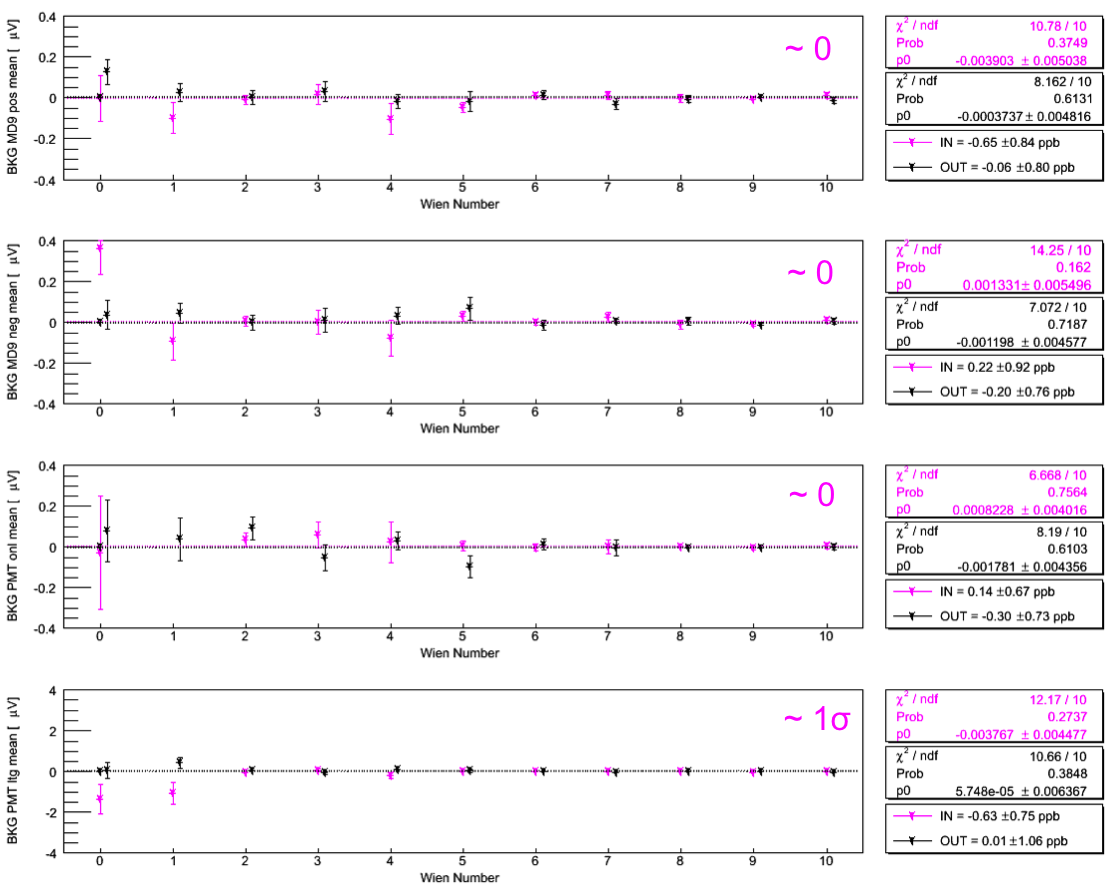
\includegraphics[width=15.0cm]{figures/pedestalDiffBkg}
	\caption
%	[Mean of the helicity correlated differences for important background detectors.]
	{Mean of the helicity correlated differences for MD9 pos, MD9 neg, PMT onl, and PMT ltg are shown in the figure (top to bottom). Helicity correlated differences for these important background detectors from Hel\_Tree are zero within $\sim$1$\sigma$ for averaged over each wien.}
	\label{fig:pedestalDiffBkg}
\end{figure}
\end{singlespace}

\begin{singlespace}
\begin{figure}[!h]
	\centering
	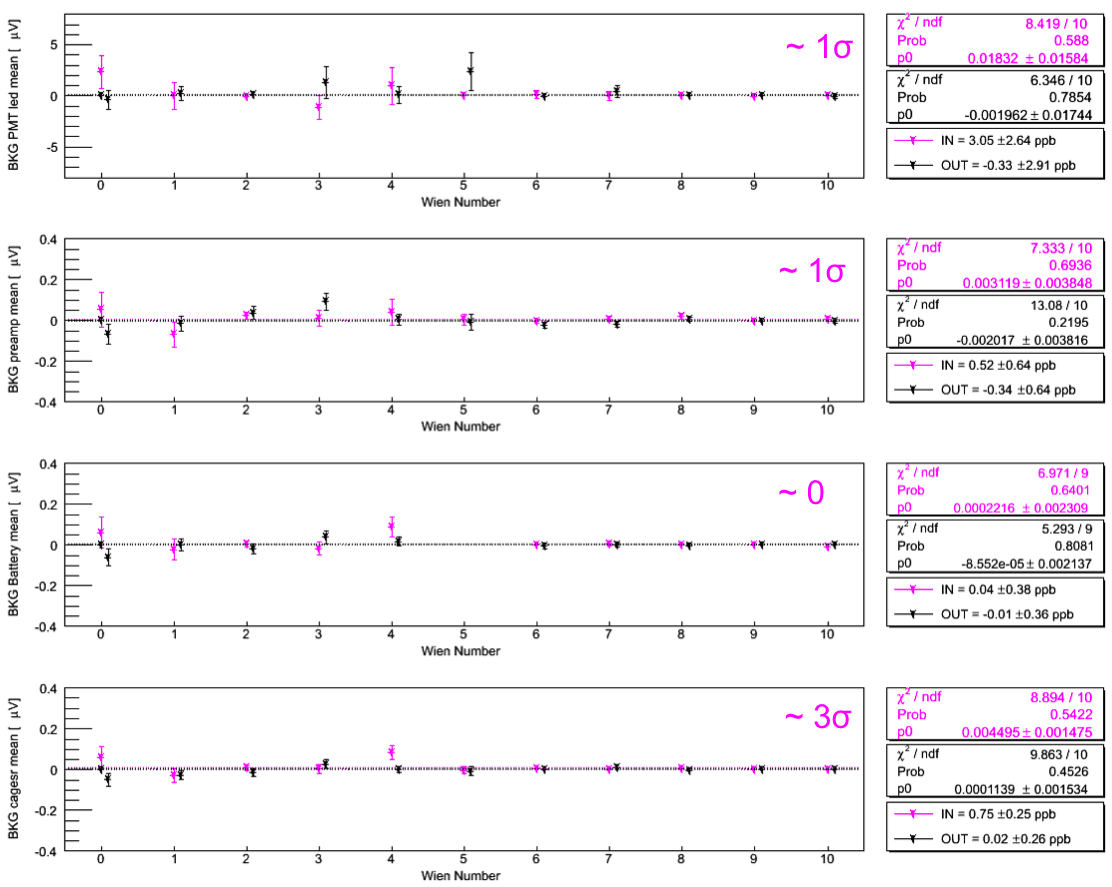
\includegraphics[width=15.0cm]{figures/pedestalDiffBkgOther}
	\caption
%	[Mean of the helicity correlated differences for other background detectors.]
	{Mean of the helicity correlated differences for PMT led, preamp, battery, and cages source are shown in the figure (top to bottom). Helicity correlated differences for these important background detectors from Hel\_Tree are zero within $\sim$3$\sigma$ for averaged over each wien.}
	\label{fig:pedestalDiffBkgOther}
\end{figure}
\end{singlespace}

\begin{singlespace}
\begin{figure}[!h]
	\centering
	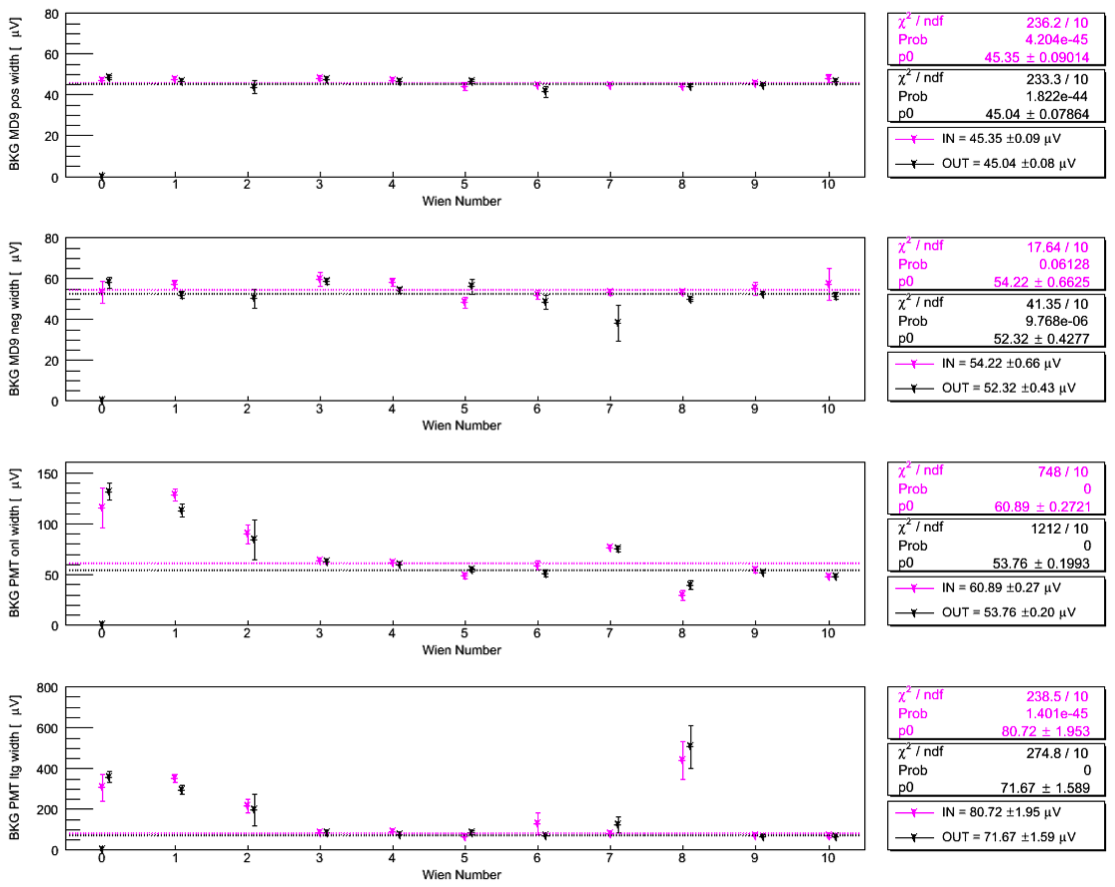
\includegraphics[width=15.0cm]{figures/pedestalDiffBkgWidth}
	\caption
%	[Width of the helicity correlated differences for important background detectors.]
	{Width of the helicity correlated differences for MD9 pos, MD9 neg, PMT onl, and PMT ltg are shown in the figure (top to bottom).}
	\label{fig:pedestalDiffBkgWidth}
\end{figure}
\end{singlespace}

\begin{singlespace}
\begin{figure}[!h]
	\centering
	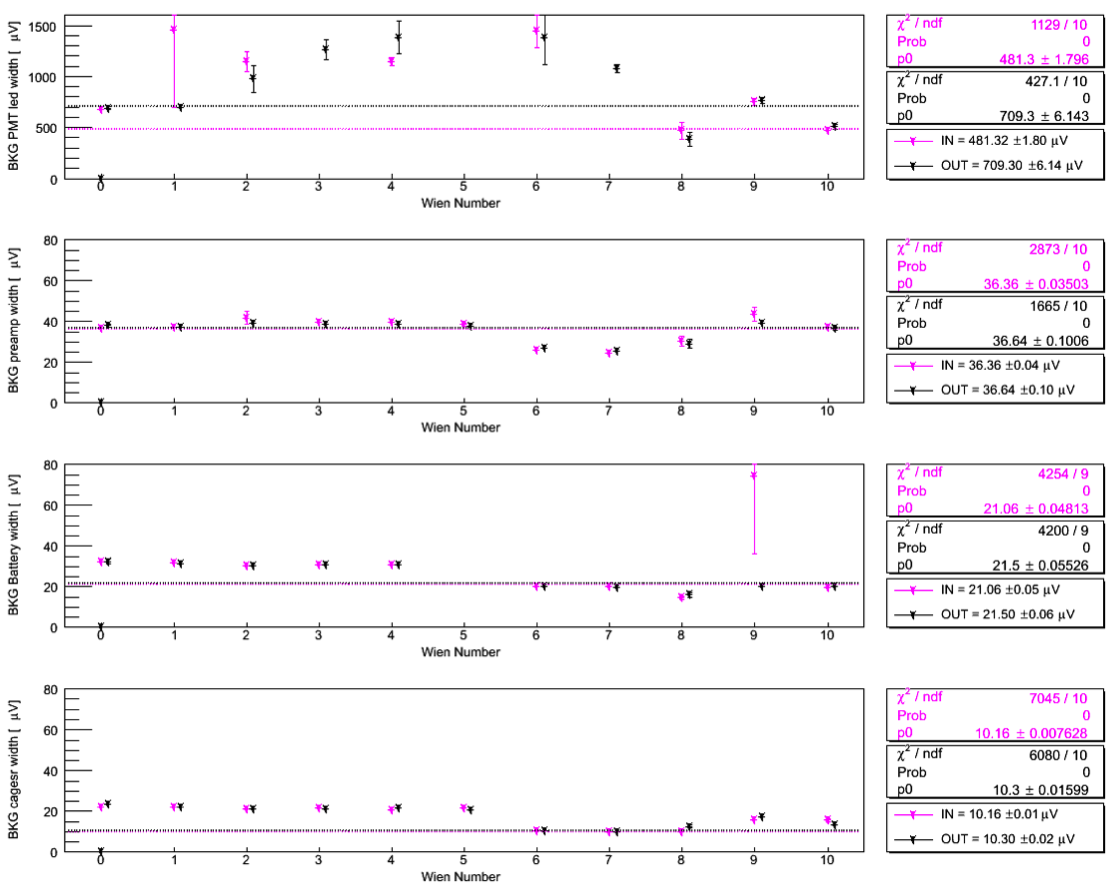
\includegraphics[width=15.0cm]{figures/pedestalDiffBkgOtherWidth}
	\caption
%	[Width of the helicity correlated differences for other background detectors.]
	{Width of the helicity correlated differences for PMT led, preamp, battery, and cages source are shown in the figure (top to bottom).}
	\label{fig:pedestalDiffBkgOtherWidth}
\end{figure}
\end{singlespace}
